\documentclass[14pt]{extbook}
\usepackage{multicol, enumerate, enumitem, hyperref, color, soul, setspace, parskip, fancyhdr} %General Packages
\usepackage{amssymb, amsthm, amsmath, bbm, latexsym, units, mathtools} %Math Packages
\everymath{\displaystyle} %All math in Display Style
% Packages with additional options
\usepackage[headsep=0.5cm,headheight=12pt, left=1 in,right= 1 in,top= 1 in,bottom= 1 in]{geometry}
\usepackage[usenames,dvipsnames]{xcolor}
\usepackage{dashrule}  % Package to use the command below to create lines between items
\newcommand{\litem}[1]{\item#1\hspace*{-1cm}\rule{\textwidth}{0.4pt}}
\pagestyle{fancy}
\lhead{Makeup Progress Quiz -1}
\chead{}
\rhead{Version A}
\lfoot{7547-2949}
\cfoot{}
\rfoot{Fall 2020}
\begin{document}

\begin{enumerate}
\litem{
Solve the modeling problem below, if possible.
\begin{center}
    \textit{ A new virus is spreading throughout the world. There were initially 8 many cases reported, but the number of confirmed cases has doubled every 2 days. How long will it be until there are at least 10000 confirmed cases? }
\end{center}
\begin{enumerate}[label=\Alph*.]
\item \( \text{About } 15 \text{ days} \)
\item \( \text{About } 21 \text{ days} \)
\item \( \text{About } 6 \text{ days} \)
\item \( \text{About } 7 \text{ days} \)
\item \( \text{There is not enough information to solve the problem.} \)

\end{enumerate} }
\litem{
Determine the appropriate model for the graph of points below.
\begin{center}
    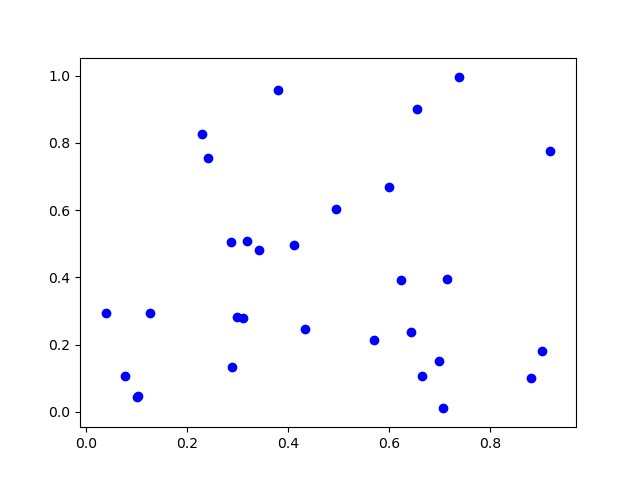
\includegraphics[width=0.5\textwidth]{../Figures/identifyModelGraph12CopyA.png}
\end{center}
\begin{enumerate}[label=\Alph*.]
\item \( \text{Exponential model} \)
\item \( \text{Logarithmic model} \)
\item \( \text{Non-linear Power model} \)
\item \( \text{Linear model} \)
\item \( \text{None of the above} \)

\end{enumerate} }
\litem{
For the scenario below, use the model for the volume of a cylinder as $V = \pi r^2 h$ to find the coefficient for the model of the new volume $V_{	ext{new}} = k r^2 h$.
\begin{center}
    \textit{ Pepsi wants to increase the volume of soda in their cans. They've decided to increase the radius by 13 percent and increase the height by 19 percent. They want to model the new volume based on the radius and height of the original cans. }
\end{center}
\begin{enumerate}[label=\Alph*.]
\item \( k = 0.00321 \)
\item \( k = 4.77368 \)
\item \( k = 0.01009 \)
\item \( k = 1.51951 \)
\item \( \text{None of the above.} \)

\end{enumerate} }
\litem{
Determine the appropriate model for the graph of points below.
\begin{center}
    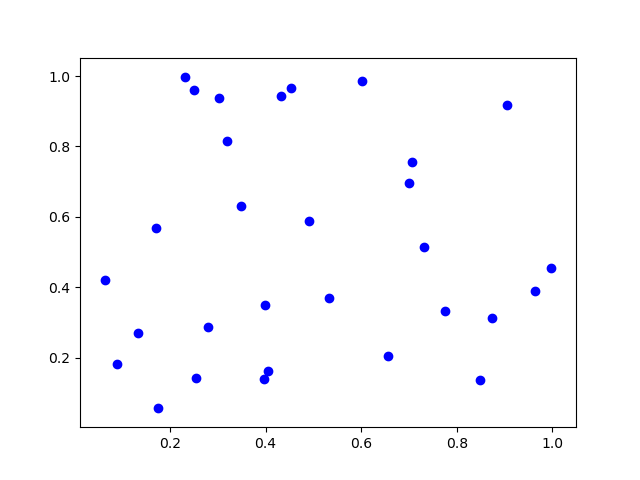
\includegraphics[width=0.5\textwidth]{../Figures/identifyModelGraph12A.png}
\end{center}
\begin{enumerate}[label=\Alph*.]
\item \( \text{Linear model} \)
\item \( \text{Exponential model} \)
\item \( \text{Non-linear Power model} \)
\item \( \text{Logarithmic model} \)
\item \( \text{None of the above} \)

\end{enumerate} }
\litem{
Solve the modeling problem below, if possible.
\begin{center}
    \textit{ In CHM2045L, Brittany created a 20 liter 24 percent solution of chemical $\chi$ using two different solution percentages of chemical $\chi$. When she went to write her lab report, she realized she forgot to write the amount of each solution she used! If she remembers she used 12 percent and 27 percent solutions, what was the amount she used of the 12 percent solution? }
\end{center}
\begin{enumerate}[label=\Alph*.]
\item \( 10.00 \)
\item \( 9.13 \)
\item \( 4.00 \)
\item \( 16.00 \)
\item \( \text{There is not enough information to solve the problem.} \)

\end{enumerate} }
\litem{
For the scenario below, use the model for the volume of a cylinder as $V = \pi r^2 h$.
\begin{center}
    \textit{ Pringles wants to add 38 \text{percent} more chips to their cylinder cans and minimize the design change of their cans. They've decided that the best way to minimize the design change is to increase the radius and height by the same percentage. What should this increase be? }
\end{center}
\begin{enumerate}[label=\Alph*.]
\item \( \text{About } 19 \text{ percent} \)
\item \( \text{About } 3 \text{ percent} \)
\item \( \text{About } 11 \text{ percent} \)
\item \( \text{About } 17 \text{ percent} \)
\item \( \text{None of the above} \)

\end{enumerate} }
\litem{
For the information provided below, construct a linear model that describes her total budget, $B$, as a function of the number of months, $x$ she is at UF.
\begin{center}
    \textit{ Aubrey is a college student going into her first year at UF. She will receive Bright Futures, which covers her tuition plus a \$400 educational expense each year. Before college, Aubrey saved up \$5000. She knows she will need to pay \$700 in rent a month, \$80 for food a week, and \$40 in other weekly expenses. }
\end{center}
\begin{enumerate}[label=\Alph*.]
\item \( B(x) = 5000 x + 400 \)
\item \( B(x) = 5400 - 1180 x \)
\item \( B(x) = 5400 - 820 x \)
\item \( B(x) = 400 x + 5000 \)
\item \( \text{None of the above.} \)

\end{enumerate} }
\litem{
Solve the modeling problem below, if possible.
\begin{center}
    \textit{ A new virus is spreading throughout the world. There were initially 4 many cases reported, but the number of confirmed cases has doubled every 5 days. How long will it be until there are at least 100000 confirmed cases? }
\end{center}
\begin{enumerate}[label=\Alph*.]
\item \( \text{About } 25 \text{ days} \)
\item \( \text{About } 51 \text{ days} \)
\item \( \text{About } 28 \text{ days} \)
\item \( \text{About } 74 \text{ days} \)
\item \( \text{There is not enough information to solve the problem.} \)

\end{enumerate} }
\litem{
Solve the modeling problem below, if possible.
\begin{center}
    \textit{ In CHM2045L, Brittany created a 22 liter 7 percent solution of chemical $\chi$ using two different solution percentages of chemical $\chi$. When she went to write her lab report, she realized she forgot to write the amount of each solution she used! If she remembers she used 5 percent and 16 percent solutions, what was the amount she used of the 5 percent solution? }
\end{center}
\begin{enumerate}[label=\Alph*.]
\item \( 4.00 \)
\item \( 11.00 \)
\item \( 18.00 \)
\item \( 13.63 \)
\item \( \text{There is not enough information to solve the problem.} \)

\end{enumerate} }
\litem{
For the scenario below, use the model for the volume of a cylinder as $V = \pi r^2 h$.
\begin{center}
    \textit{ Pringles wants to add 36 \text{percent} more chips to their cylinder cans and minimize the design change of their cans. They've decided that the best way to minimize the design change is to increase the radius and height by the same percentage. What should this increase be? }
\end{center}
\begin{enumerate}[label=\Alph*.]
\item \( \text{About } 11 \text{ percent} \)
\item \( \text{About } 17 \text{ percent} \)
\item \( \text{About } 18 \text{ percent} \)
\item \( \text{About } 3 \text{ percent} \)
\item \( \text{None of the above} \)

\end{enumerate} }
\end{enumerate}

\end{document}